\section{The quantum shape: floor, real-state theorem, fossil, nonlinear survival}\label{rep:quantum-shape}

The aspect modes of Sec.~\ref{rA:sh-modes} are unstable, so their quantum state at the turning point decides the shape of the torus afterward.
The uncertainty principle sets a floor on their outgoing spread, which we obtain in closed form: $\sfloor=0.104$ per aspect mode for the Standard Model. %
We prove that the correlation of an aspect mode grows monotonically, so the shape state is real at most once, and that the outgoing spread grows quickly with the distance of that moment from the turn.
Including nonlinear evolution, we find that, for a real Gaussian state, survival of the shape on both branches with probability $90\%$ ($99\%$) requires the moment of reality to lie within $0.35/h$ ($0.24/h$) of the turn. %
The natural state, real at the turn (assumption~\ref{assump:A8}), freezes into a quantum fossil, an almost rectangular box whose longest and shortest sides typically differ by $16$--$18\%$; every state real at the turn leaves a fossil at least at the floor. %
The Euclidean continuation of the turning point does not select the state.
Sections~\ref{rA:s-quantization}--\ref{rA:s-natural} quantize the modes and derive the floor and the natural state, Sec.~\ref{rA:s-theorem} proves the real-moment theorem and combines it with nonlinear survival into the conditional theorem, Sec.~\ref{rA:s-equivalent} relates reality to the Wheeler--DeWitt wave function, Sec.~\ref{rA:s-fossil} gives the fossil and its error budget, Sec.~\ref{rA:s-nonlinear} the nonlinear evolution and its corrections, and Sec.~\ref{rA:s-euclid} the Euclidean continuation.

\subsection{Quantization of the shape modes}
\label{rA:s-quantization}

The canonical momentum of mode $A$ is $P_A=\MPbar^2L^3\dot\beta_A$ (Eq.~\eqref{eq:rA-PA}), and $[\beta_A,P_B]=i\delta_{AB}$.
On the $A_s$-calibrated plateau the rate of the turning-point solution is $\rAHeff=[V(\phi_b)/3]^{1/2}/\MPbar=0.98949\,h$; it replaces $h$ in Eq.~\eqref{eq:rA-shapeode} there. %
We rescale the momentum, $\Pi_A=P_A/p_0$ with $p_0=3\MPbar^2\rAHeff\Lb^3/2^{3/2}$, so that in units of $\Lb$ and $1/\rAHeff$ the mode obeys $\dot\beta=c\,\Pi/L^3$ with $c=3/2^{3/2}$ and the second fundamental solution of Sec.~\ref{rA:sh-transfer} has unit incoming $\Pi$.
Then
\begin{equation}
[\beta_A,\Pi_B]=2i\delta\,\delta_{AB},\qquad
\delta=\frac{1}{2p_0}=\frac{\sqrt2}{3X},\qquad X\equiv\MPbar^2\Lb^3\rAHeff .
\label{eq:rA-delta}
\end{equation}
The constant $\delta$ plays the role of $\hbar$ for the shape.
Times in this chapter are in units of $1/\rAHeff$, so $h|t|$ below stands for $\rAHeff|t|$; in units of the plateau parameter, $1/h$, they are $1\%$ larger. %
With $\Lb^4=C_{\rm eff}/3\MPbar^2\rAHeff^2$,
\begin{equation}
X=\Big(\frac{\rANeff\rAgam}{3}\Big)^{3/4}\Big(\frac{\MPbar}{\rAHeff}\Big)^{1/2},
\end{equation}
so fewer light fields give a smaller $X$ and a larger $\delta$.
For the Standard Model with $\fzm=0.30$, $X=2282.5$ and $\delta=2.065\times10^{-4}$. %
A linear mode maps incoming to outgoing data by the symplectic matrix $\rATm$ of Sec.~\ref{rA:sh-transfer}, $(\beta_+,\Pi_+)=\rATm(\beta_-,\Pi_-)$, as an operator identity.

\subsection{A floor from the uncertainty principle}
\label{rA:s-floor}

Since $\beta_+=\rATm_{11}\beta_-+\rATm_{12}\Pi_-$, the commutator of the incoming and outgoing amplitudes is $[\beta_-,\beta_+]=\rATm_{12}[\beta_-,\Pi_-]=2i\delta\rATm_{12}$.
Robertson's inequality then gives, in every state,
\begin{equation}
\rAVar\,\beta_-\,\rAVar\,\beta_+\geq\tfrac14\big|\langle[\beta_-,\beta_+]\rangle\big|^2=\delta^2\rATm_{12}^2 .
\end{equation}

\begin{rAlemma}[All-time bound]\label{lem:rA-alltime}
For an anti-restoring mode, $\max_t\rAVar\,\beta(t)\geq\delta|\rATm_{12}|$ in every state, and the bound is attained by a pure Gaussian.
\end{rAlemma}

\begin{rAproof}
The endpoint inequality gives $\max_\pm\rAVar\,\beta_\pm\geq\delta|\rATm_{12}|$, and the endpoint variances are limits of $\rAVar\,\beta(t)$.
For attainment, let $u,v$ solve the anti-restoring equation $(m\dot\beta)^{\boldsymbol\cdot}=k\beta$, $m>0$, $k\geq0$, with $u(t_-)=1$, $u(t_+)=0$, $v(t_-)=0$ and $v(t_+)=1$, so that $\beta(t)=u(t)\beta_-+v(t)\beta_+$ for every solution.
The maximum principle gives $u,v\geq0$ and $u+v\leq1$: at an interior negative minimum of $u$, or an interior maximum of $u+v$ above one, $m\ddot\beta$ and $k\beta$ would have opposite signs.
For the pure Gaussian with equal endpoint variances $\delta|\rATm_{12}|$ and zero symmetrized endpoint covariance, which saturates the Robertson--Schr\"odinger inequality for $(\beta_-,\beta_+)$,
\begin{equation}
\rAVar\,\beta(t)=\delta|\rATm_{12}|\,(u^2+v^2)\leq\delta|\rATm_{12}|\,(u+v)^2\leq\delta|\rATm_{12}| ,
\end{equation}
so the endpoint bound is attained at all times.
\end{rAproof}

The shape cannot stay narrower than
\begin{equation}
\sfloor\equiv(\delta|\rATm_{12}|)^{1/2}
\end{equation}
throughout, however it is prepared.

\paragraph{Closed form.}
Let $M$ be the transfer from the turning point to the far future.
Because the background is time symmetric, the full transfer is $\rATm=M\mathsf RM^{-1}\mathsf R$ with $\mathsf R={\rm diag}(1,-1)$, Eq.~\eqref{eq:rA-Tsym}, so $\rATm_{12}=2m_{11}m_{12}$.
The connection formulas of Sec.~\ref{rA:sh-transfer} give $\rATm_{11}=\rAGain(\kappa)$ and
\begin{equation}
\rATm_{12}=\frac{\Gamma(\tfrac74)\Gamma(\tfrac34)}{|\Gamma(\tfrac54+i\mu)|^2},\qquad
\mu=\frac{\sqrt{4\kappa-1}}{4}.
\label{eq:rA-T12b}
\end{equation}
The floor therefore has the closed form
\begin{equation}
\sfloor^2=\frac{\sqrt2\,\Gamma(\tfrac74)\Gamma(\tfrac34)}{3\,|\Gamma(\tfrac54+i\mu_E)|^2\,\MPbar^2\Lb^3\rAHeff}=\frac{K(\kappa_E)}{X},\qquad K(\kappa)=\frac{\sqrt2\,\Gamma(\tfrac74)\Gamma(\tfrac34)}{3|\Gamma(\tfrac54+i\mu)|^2},
\label{eq:rA-floor}
\end{equation}
where $\mu_E$ is the value of $\mu$ at $\kappa_E$.
In units of $X$, $K=24.550$ at $\kappa_E=19.32$ and $20.320$ at $18.0$. %
For the Standard Model with $\fzm=0.30$, $\kappa_E=19.32$ and $\rATm_{12}=52.1$, so $\sfloor=0.1037$; at next order, $\kappa_E=18.0$ and $\fzm\simeq0.28$, $X$ grows by $[(1-0.28)/(1-0.30)]^{3/4}$ and the floor is $0.0934$. %

\subsection{The natural state}
\label{rA:s-natural}

At the turning point an anti-restoring mode is an inverted oscillator with mass $m_{\rm sh}=\MPbar^2\Lb^3$ and frequency $|\omega|=\sqrt{\kappa}\,\rAHeff=(|\kappa|v_b/3)^{1/2}h$, where $v_b=V(\phi_b)/\MPbar^2h^2=3(\rAHeff/h)^2\simeq2.94$. %
Its natural local width, $s_{\rm nat}=1/(2m_{\rm sh}|\omega|)=1/(2X\sqrt\kappa)$ in variance, is the width whose spreading matches the instability.

A real Gaussian at the turning point with $\rAVar\,\beta_0=s$ has $\rAVar\,\Pi_0=\delta^2/s$ and no correlation, and $\beta_+=m_{11}\beta_0+m_{12}\Pi_0$ gives
\begin{equation}
\rAVar\,\beta_+=m_{11}^2s+\frac{m_{12}^2\delta^2}{s}=\delta|\rATm_{12}|\,\frac{x+x^{-1}}2,\qquad x=\frac{s}{s_*},
\label{eq:rA-family}
\end{equation}
with $s_*=|m_{12}/m_{11}|\,\delta$; the second form uses $\rATm_{12}=2m_{11}m_{12}$.
The all-time optimum of Lemma~\ref{lem:rA-alltime} is exactly this state at $s=s_*$, where $\rAVar\,\beta_\pm=\delta|\rATm_{12}|$.
For the Standard Model aspect modes $s_*=4.83\times10^{-5}$ and $s_{\rm nat}=4.98\times10^{-5}$, so $x=1.032$ and the natural state lies $(x+x^{-1})/2-1=0.05\%$ above the floor in variance; for free fields the excess is $0.12\%$ [Fig.~\ref{fig:rA-turning-state}(c)]. %
For strongly anti-restoring modes the optimal width is thus set by the instability itself, and Sec.~\ref{rA:s-equivalent} shows that it is the time-symmetric Gaussian of minimal energy variance.
The restoring angle modes sit a factor $1.35$ above their endpoint floor in variance, and their outgoing widths remain below $0.007$. %
At the turn the natural aspect state has $\beta_{\rm rms}=s_{\rm nat}^{1/2}=0.0071$. %

\subsection{When the shape state is real}
\label{rA:s-theorem}

The floor and Eq.~\eqref{eq:rA-family} take the shape state to be real at the turning point, and that state cannot be inherited from the contracting branch.

\paragraph{Freezing.}
Along the solution the local frequency of mode $A$ is $\omega_A=\sqrt{|\kappa_A|}\,h\,{\rm sech}\,2ht$ and $|H|=h|\tanh2ht|$, so
\begin{equation}
\frac{\omega_A}{|H|}=\frac{\sqrt{|\kappa_A|}}{|\sinh2ht|}
\end{equation}
identically.
The shape modes freeze from $h|t|=\tfrac12{\rm arsinh}\sqrt{|\kappa_A|}$, which is $1.093$ for the aspect and $0.911$ for the angle modes at $\fzm=0.30$, $0.75$ and $0.58$ e-folds of expansion, $\ln(L/\Lb)=\tfrac12\ln\cosh2ht$, before the turn. %
The angle modes accumulate a total phase $\int\omega\,dt=\sqrt{|\kappa_{T_2}|}\,\pi/2=4.73<2\pi$ over the whole window, so they have no usable asymptotic vacuum either. %

\paragraph{The far past.}
On the plateau the anisotropic stiffness of every sector of our matter content is suppressed by the slow-roll parameter, so the modes have no oscillating asymptotic vacuum in the far past.
In a far past dominated by a component with energy $\propto L^{m_d}$, a shape stiffness from a component with energy $\propto L^{m_s}$ gives $\omega^2/H^2\propto L^{m_s-m_d}$.
In e-fold time $N=\ln L$ the mode equation is $\beta''+\tfrac12(3+m_d)\beta'+(\omega^2/H^2)\beta=0$, because $\dot H/H^2=(m_d-3)/2$.
The modes then have an oscillating (WKB) vacuum for $m_s>m_d$, freeze for $m_s<m_d$, and for $m_s=m_d$ oscillate if and only if $\omega^2/H^2>[(3+m_d)/4]^2$.
On the plateau, $m_d=3$, $\omega^2/H^2=3(K_s/e_s)\Omega_s$, with $\Omega_s$ the energy share of the sector that supplies the stiffness $K_s$, so slow roll limits it to $\mathcal O(\epsilon_V)\ll9/4$.
Sectors that evade this, such as vector fields with an inflaton-dependent kinetic function~\cite{Watanabe:2009ct}, non-abelian gauge fields with a vacuum expectation value~\cite{Maleknejad:2011jw,Adshead:2012kp}, the shear modulus of solid inflation~\cite{Endlich:2012pz} or domain walls wrapping a two-cycle, are absent from the Standard Model with a plateau inflaton.
A state set on the contracting branch is therefore set where the modes are already frozen.
We now ask what reality of the state does to the shape, if it holds at any moment.

\subsubsection{The real-moment theorem}
\label{rA:s-realmoment}

We call the shape state real at $t_x$ if the symmetrized correlation
\begin{equation}
C(t)\equiv\tfrac12\langle\{\delta\beta,\delta\Pi\}\rangle
\end{equation}
of an aspect mode vanishes there, with $\delta\beta=\beta-\langle\beta\rangle$ and $\delta\Pi=\Pi-\langle\Pi\rangle$.
A real wave function has this property at the moment where it is real, and so has any state invariant under time reversal about $t_x$.

\begin{rAtheorem}[Real moment]\label{thm:rA-real}
For the linearized dynamics of Eq.~\eqref{eq:rA-shapeode}, for an aspect mode ($\kappa_E>0$) in any state, pure or mixed, Gaussian or not, $C(t)$ increases strictly with $t$.
The shape state is therefore real at most at one instant $t_x$, and every state is real once [$C(-\infty)<0<C(+\infty)$], never real and outgoing [$C\geq0$ throughout], or never real and incoming [$C\leq0$ throughout].
If the state is real at $t_x$, the larger of the two outgoing variances obeys
\begin{equation}
\begin{gathered}
\max_\pm\rAVar\,\beta_\pm\geq G(|t_x|)\,\delta|\rATm_{12}|,\\
G(|t_x|)=\frac{|M_{11}M_{12}|_{-|t_x|\to\infty}}{|M_{11}M_{12}|_{0\to\infty}},
\end{gathered}
\label{eq:rA-Gtx}
\end{equation}
where the subscripts give the interval of the transfer $M$.
A state that is never real has $\max_\pm\rAVar\,\beta_\pm\geq2\rAGain(\kappa_E)\,\delta|\rATm_{12}|$ and $\rAVar\,\beta_E(0)\geq2m_{12}m_{22}\delta$.
\end{rAtheorem}

\begin{rAproof}
In the units of this chapter a shape mode obeys $\dot\beta=c\,\Pi/L^3$ and $\dot\Pi=(\kappa/c)\,L^3{\rm sech}^2(2t)\,\beta$.
\emph{Monotonicity.} For linear dynamics the Ehrenfest relations close on the second moments: the means follow the classical equations, and the fluctuations $\delta\beta$, $\delta\Pi$ obey the same linear equations.
Hence $\tfrac{d}{dt}\{\delta\beta,\delta\Pi\}=\{\dot{\delta\beta},\delta\Pi\}+\{\delta\beta,\dot{\delta\Pi}\}=2(c/L^3)\delta\Pi^2+2(\kappa/c)L^3{\rm sech}^2(2t)\,\delta\beta^2$, and
\begin{equation}
\frac{dC}{dt}=\frac{c}{L^3}\,\rAVar\,\Pi+\frac{\kappa_EL^3}{c}\,{\rm sech}^2(2t)\,\rAVar\,\beta>0
\label{eq:rA-dCdt}
\end{equation}
in any state, pure or mixed, Gaussian or not, since $\rAVar\,\Pi>0$ by the uncertainty relation.
Both terms decay at least as $e^{-|t|}$, because $L^3\propto e^{3|t|}$, ${\rm sech}^2\propto e^{-4|t|}$ and the frozen variances tend to constants; so $C(\pm\infty)$ are finite, and a strictly increasing $C$ vanishes at most once.
\emph{Bound.} Let $M=M(t_{\rm ref}\to\infty)$; since $\kappa_E>0$, $M_{11}$ and $M_{12}$ are positive.
If $C(t_{\rm ref})\geq0$, then
\begin{equation}
\begin{split}
\rAVar\,\beta_+&=M_{11}^2\rAVar\,\beta+2M_{11}M_{12}C+M_{12}^2\rAVar\,\Pi\\
&\geq2M_{11}M_{12}\sqrt{\rAVar\,\beta\,\rAVar\,\Pi}\geq2M_{11}M_{12}\,\delta,
\end{split}
\end{equation}
by the arithmetic--geometric mean inequality and the Robertson--Schr\"odinger inequality $\rAVar\,\beta\,\rAVar\,\Pi-C^2\geq\delta^2$.
With $t_{\rm ref}=t_x\leq0$ and $\delta|\rATm_{12}|=2m_{11}m_{12}\delta$ this is Eq.~\eqref{eq:rA-Gtx}; for $t_x>0$ the reflection $t\to-t$, $\Pi\to-\Pi$ exchanges the branches, and the bound applies to the past one.
As $t_{\rm ref}\to-\infty$, $M_{11}M_{12}\to\rATm_{11}\rATm_{12}$, so $G(\infty)=\rATm_{11}\rATm_{12}/(m_{11}m_{12})=2\rAGain(\kappa_E)$.
An outgoing never-real state has $C\geq0$ at all times, which gives $\rAVar\,\beta_+\geq2\rAGain\,\delta|\rATm_{12}|$; an incoming one gives the same bound on $\rAVar\,\beta_-$ by reflection.
\emph{Width condition.} With $M=M(0\to\infty)$ the covariance transforms as $\Sigma_+=M\Sigma M^{\mathsf T}$, so
\begin{equation}
C(+\infty)=m_{11}m_{21}\rAVar\,\beta+(m_{11}m_{22}+m_{12}m_{21})C+m_{12}m_{22}\rAVar\,\Pi .
\end{equation}
At fixed $V\equiv\rAVar\,\beta(0)$ we minimize over $C(0)$ and $\rAVar\,\Pi\geq(\delta^2+C^2)/V$.
The minimum over $C$ lies at $C=-(m_{11}m_{22}+m_{12}m_{21})V/(2m_{12}m_{22})$, and with $(m_{11}m_{22}+m_{12}m_{21})^2=1+4m_{11}m_{12}m_{21}m_{22}$, from $\det M=1$, it is
\begin{equation}
\min C(+\infty)=\frac{m_{12}m_{22}\delta^2}{V}-\frac{V}{4m_{12}m_{22}} ,
\end{equation}
and the mirror statement holds for $C(-\infty)$.
An incoming never-real state needs $C(+\infty)\leq0$, which is possible only if $V\geq2m_{12}m_{22}\delta$; the outgoing case follows by reflection.
The bound uses only second moments and holds for mixed and non-Gaussian states.
\end{rAproof}

The proof uses only the linear equations of motion.
Fifty random covariance matrices confirm the monotonic increase numerically. %
That the correlation of an inverted-oscillator mode grows with time is the familiar squeezing of cosmological perturbations~\cite{Polarski:1995jg}; what the theorem adds is that the real moment is unique and, through Eq.~\eqref{eq:rA-Gtx}, that its distance from the turn decides whether the shape survives on both branches.
For the Standard Model at $\fzm=0.30$ the width condition reads $\rAVar\,\beta_E(0)\geq157.9\,\delta$, and $128.1\,\delta$ at next order. %

\paragraph{Numbers.}
For the Standard Model, $G=2.395$, $8.263$, $45.10$ and $313.8$ at $h|t_x|=0.1$, $0.25$, $0.5$ and $1$, $385.6$ at the onset of freezing, and $2\rAGain(\kappa_E)=1348$ as $|t_x|\to\infty$ [Fig.~\ref{fig:rA-turning-state}(d)]. %
Table~\ref{tab:rA-G} lists $G$ and the single-branch future bound $G_+$.
A real state set in the frozen region of the contracting branch is therefore amplified at least $19.6$-fold in rms, and a never-real state at least $36.7$-fold, to $\sigma_E\gtrsim3.8$. %
A never-real state must also be wide at the turn, $\beta_{\rm rms}(0)\geq(157.9\,\delta)^{1/2}=0.181$, with a variance $654$ times the natural one. %
Because the background is time symmetric, a moment of reality before the turn bounds the future branch and one after the turn bounds the past branch.
In the single-branch reading, in which only $t>0$ is physical, a state real after the turn can leave the future branch below the floor, by factors $0.417$, $0.120$, $0.0214$ and $0.0022$ at $ht_x=0.1$, $0.25$, $0.5$ and $1$. %
The floor is thus an all-time bound, not a bound on the future branch alone.

\begin{table}[tbp]
\centering
\caption{Amplification of the larger outgoing aspect variance, in units of the floor, for a state real at $t_x$, Eq.~\eqref{eq:rA-Gtx}, at leading ($\kappa_E=19.32$) and next order ($\kappa_E=18.0$), and the lower bound $G_+$ on the future branch alone when $t_x>0$. F marks the onset of freezing, $h|t_x|=1.093$ ($1.076$ at next order).}
\label{tab:rA-G}
\begin{tabular}{lccc}
\toprule
$h|t_x|$ & $G$ & $G$, next order & $G_+$\\
\midrule
0.05 & 1.551 & 1.528 & 0.645\\ %
0.1 & 2.395 & 2.324 & 0.417\\ %
0.25 & 8.263 & 7.679 & 0.120\\ %
0.35 & 17.35 & 15.71 & 0.057\\ %
0.5 & 45.10 & 39.51 & 0.0214\\ %
1 & 313.8 & 257.2 & 0.0022\\ %
F & 385.6 & 303.4 & 0.0016\\ %
2 & 961.7 & 761.1 & $9.5\times10^{-5}$\\ %
$\infty$ & 1347.65 & 1058.34 & 0\\ %
\bottomrule
\end{tabular}
\end{table}

\paragraph{Other classes of states.}
A pure Gaussian at the turn with the optimal width $s_*$ and correlation $C=\varphi\delta$ has $\rAVar\,\Pi=\delta^2(1+\varphi^2)/s_*$, and the transfer gives
\begin{equation}
\rAVar\,\beta(\pm\infty)=\delta|\rATm_{12}|\Big(1\pm\varphi+\frac{\varphi^2}2\Big)
\end{equation}
exactly, the sign of the middle term changing under the reflection $\Pi\to-\Pi$.
A scan of $|\varphi|\leq50$ finds every member real once, at $h|t_x|\leq0.098$, consistent with the width condition; in the single-branch reading the future branch reaches its minimum, half the floor, at $\varphi=-1$. %
A Gaussian with a phase at the turn is therefore real once, within $0.098/h$ of the turn, for every phase we scanned. %
A first-order adiabatic Gaussian set at $t_{\rm in}<0$, with its width fixed by $W=\max(\omega_{\rm loc},|H|)$ and $\omega_{\rm loc}=\sqrt{\kappa}/\cosh2t$, has $C(t_{\rm in})>0$ on the contracting branch and is never real on $[t_{\rm in},\infty)$.
Its linear fossil is $8.77$, $51.8$ and $487$ floors for $t_{\rm in}=-0.25$, $-0.5$ and $-1$, against $8.26$, $45.1$ and $314$ for the optimal real state at the same moment. %

\subsubsection{Survival and the conditional theorem}
\label{rA:s-conditional}

The linear bound turns into a constraint on the moment of reality once nonlinear evolution is included, because large outgoing deformations end the shape (Sec.~\ref{rA:s-nonlinear}).

\paragraph{Method.}
We prepared at $t_x$ the real Gaussian of optimal width, the best case of the real family at linear order, and sampled its Wigner function.
For each $\tau=|t_x|$ we sample the optimal-width real Gaussian at $t_x=-\tau$, each mode with variance $|M_{12}/M_{11}|\delta$ for the transfer $M$ from $-\tau$ to $+\infty$, and form mirror pairs.
Branch A starts at $-\tau$ with $(\beta,\Pi)$ and crosses the turn; branch B starts at $+\tau$ with $(\beta,-\Pi)$ and only expands.
Each draw was evolved through the full nonlinear equations for the volume and the five shape moduli, with the twisted Ewald forces of the AAA Standard Model and the zero-mode energy, on the turning-point solution (Sec.~\ref{rA:s-nonlinear}).
Because the equations are invariant under $t\to-t$, $H\to-H$ and the Wigner function of a real state is even in $\Pi$, the same pair gives both branches for $t_x=-\tau$ and for $t_x=+\tau$, and the two-branch survival $S_2=P(A\wedge B)$ is exactly symmetric under $t_x\to-t_x$.
In the single-branch reading the survival is $P(A)$ for $t_x=-\tau$, and $P(B)$ together with the absence of collapse of A on $[-\tau,0]$ for $t_x=+\tau$.
A direct backward integration from $+0.5$ to $-12$ reproduces the fates of the mirror construction for 8 of 8 draws and the outgoing shapes of the survivors bit for bit. %
Every failure is a finite-time collapse of one cycle after the volume has turned.
Branch B survives in every draw of every run, $0$ failures in $6912$ at leading and $768$ at next order, so $S_2$ lies within $4\times10^{-4}$ below the survival of A at $95\%$ confidence. %
For real states $S_2$ is therefore a single-branch probability, and the caveat on joint probabilities of two branches discussed for the Higgs zero mode (Sec.~\ref{rep:h-survival}) does not arise.
Seeds are declared in advance and no draw is discarded.

\paragraph{Results.}
With $2048$ draws per point, $S_2=0.9990$, $0.9868$, $0.9604$ and $0.9087$ at $h|t_x|=0.20$, $0.25$, $0.30$ and $0.35$; it falls to $0.609$ at $0.5$ and $0.152$ at $1$ [Fig.~\ref{fig:rA-survival}(b)]. %
Table~\ref{tab:rA-S2} lists $S_2$ with Wilson intervals.
The thresholds $t_*$ come from linear interpolation between neighboring nodes, with errors from $2\times10^4$ Monte Carlo draws of the Jeffreys posteriors of the nodes, and a binomial logistic fit serves as a cross-check: it gives $0.245$ at $99\%$ and $0.352$ at $90\%$. %
The levels $99\%$, $90\%$ and $50\%$ are crossed at $h|t_*|=0.237$ ($95\%$ interval $0.225$--$0.252$), $0.355\pm0.003$ and $0.631$. %
The $90\%$ crossing interpolates between the 2048-draw node at $0.35$ and a 512-draw node at $0.40$. %
An independent blind implementation, with its own model code and common random numbers over $2048$ draws per point, gives $h|t_*|=0.360\pm0.004$ at $90\%$ and $0.243\pm0.009$ at $99\%$ (Sec.~\ref{rep:v-blind}). %
At next order the $99\%$ level moves to $0.265$. %
Widening or narrowing the state by a factor of 2 at $h|t_x|=0.3$ lowers the survival from $95.7\%$ to $92.6\%$ and $91.4\%$ on the same draws; departing from the optimal width by a factor of two in either direction lowers the survival by a further $3$--$7$ percentage points, and mixed real states have larger outgoing variances by the linear bound. %
The trajectory ensemble does not represent non-Gaussian real states, whose Wigner function can be negative.

\begin{table}[tbp]
\centering
\caption{Two-branch survival $S_2$ of the optimal real Gaussian state at $t_x$, with Wilson $95\%$ intervals and the rms outgoing linear amplitude $\sigma_{\rm lin}$ of the branch that crosses the turn, at $\fzm=0.30$. Rows with 1024 and 2048 draws give the survival of the crossing branch, which equals $S_2$ to within $4\times10^{-4}$.}
\label{tab:rA-S2}
\begin{tabular}{lccc}
\toprule
$h|t_x|$ & draws & $S_2$ & $\sigma_{\rm lin}$\\
\midrule
0.15 & 1024 & 1.0000 (0.9963--1) & 0.201\\ %
0.20 & 2048 & 0.9990 (0.9964--0.9997) & 0.245\\ %
0.25 & 2048 & 0.9868 (0.9809--0.9909) & 0.297\\ %
0.30 & 2048 & 0.9604 (0.9511--0.9681) & 0.363\\ %
0.35 & 2048 & 0.9087 (0.8954--0.9204) & 0.429\\ %
0.40 & 512 & 0.816 (0.781--0.848) & 0.506\\ %
0.50 & 256 & 0.609 (0.548--0.667) & 0.728\\ %
0.70 & 256 & 0.402 (0.344--0.463) & 1.098\\ %
1.00 & 256 & 0.152 (0.113--0.201) & 1.784\\ %
1.10 & 256 & 0.117 (0.083--0.162) & 2.074\\ %
\bottomrule
\end{tabular}
\end{table}

\paragraph{States that are never real.}
States that are never real fare worse.
We evolved the extreme case: a mirror pair of states with $1.2$ and $2$ times the minimum width that never-real states need, and with extremal correlation. %
They survive on both branches in $4.3\%$ (Wilson $95\%$ interval $2.4$--$7.5\%$) and $2.7\%$ ($1.3$--$5.5\%$) of the trajectories; here both branches can fail, so these are joint frequencies of the truncated Wigner ensemble. %
In the single-branch reading the incoming member survives in $88.7\%$ and $72.3\%$ of the trajectories, but its survivors carry $\sigma_E=0.33$ and $0.44$, three to four times the floor, because nonlinearity spoils the cancellation that focuses this state at linear order. %
First-order adiabatic states on the contracting branch, never real after their preparation at $t_{\rm in}$, survive in $99.2\%$, $60.9\%$ and $12.9\%$ of the trajectories for $ht_{\rm in}=-0.25$, $-0.5$ and $-1$, no better than the optimal real state at the same moment. %
Real states set in the frozen region keep the shape in only $13$--$18\%$ of the trajectories, and the survivors carry $\sigma_E\simeq0.7$--$0.9$. %
The cases tested on the $A_s$-calibrated plateau history, amplitudes $s=1$--$10$ and real states at $ht_x=-0.5$, $-1$ and the onset of freezing, change no fate (Sec.~\ref{rA:s-nonlinear}). %

\paragraph{The conditional theorem.}
Combining Theorem~\ref{thm:rA-real} with these results gives the conditional theorem of this chapter, which we state once.

\begin{rAtheorem}[Conditional theorem]\label{thm:rA-conditional}
If the shape state is real at some instant $t_x$, then that instant is unique, and in the two-branch reading, in which both branches are physical futures of the same state, survival of the shape on both branches (equivalently, on the branch that crosses the turn) with probability of at least $90\%$ ($99\%$) requires, for a Gaussian state, $h|t_x|\lesssim0.35$ ($0.24$), on either side of the turning point. %
\end{rAtheorem}

The uniqueness and the linear bound are proved; the thresholds are numerical, with the statistical intervals given above, and refer to the best case among real Gaussian states.
The two extreme never-real states we evolved, the limit $|t_x|\to\infty$ of Theorem~\ref{thm:rA-real}, survive on both branches in $4.3\%$ and $2.7\%$ of trajectories. %
In the single-branch reading the statement constrains only $t_x<0$: real states with $0<ht_x\leq1.1$ all survive, with a fossil below the floor. %

\begin{figure}[tbp]
\centering
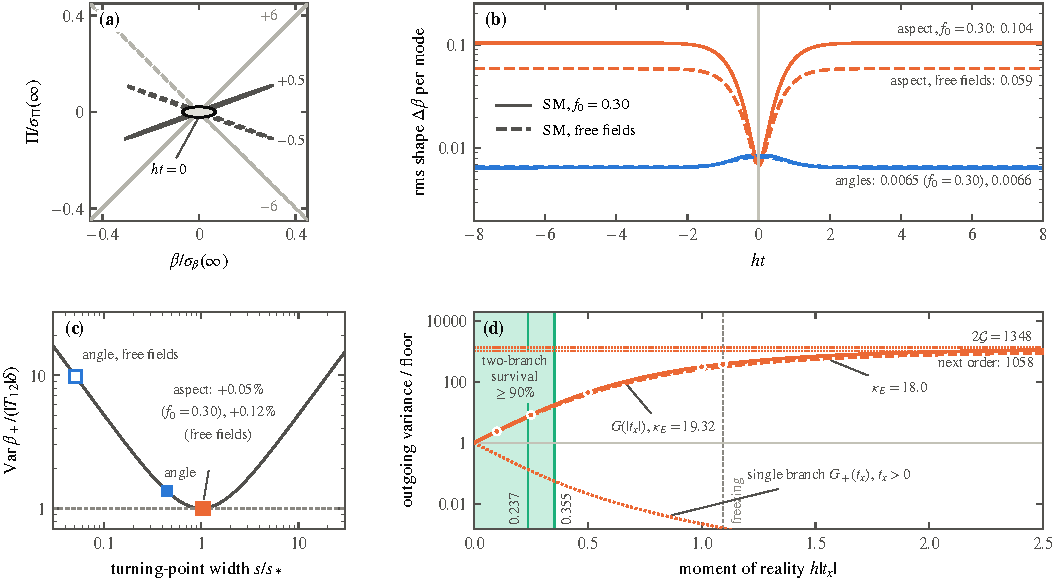
\includegraphics[width=\textwidth]{prd_turning_state}
\caption{The quantum shape through the turning point. (a)~$1\sigma$ Wigner ellipses of the natural state of a Standard Model aspect mode ($\fzm=0.30$) at $ht=0$, $\pm0.5$ and $\pm6$ (past dashed), in outgoing widths. (b)~Rms width of the aspect and angle modes versus time for $\fzm=0.30$ (solid) and free fields (dashed). (c)~Outgoing variance in units of the floor versus the turning-point width, Eq.~\eqref{eq:rA-family}; squares: natural widths (filled: $\fzm=0.30$; open: free fields). (d)~Bound $G(|t_x|)$ for a state real at $t_x$, Eq.~\eqref{eq:rA-Gtx}, at $\kappa_E=19.32$ and $18.0$ (dashed), single-branch bound $G_+$ (dotted), and two-branch survival thresholds $h|t_*|=0.237$ ($99\%$) and $0.355$ ($90\%$, shaded).} %
\label{fig:rA-turning-state}
\end{figure}

\subsection{Time symmetry and the Wheeler--DeWitt wave function}
\label{rA:s-equivalent}

Reality of the shape state at the turn is a statement about the wave function of the universe, and three results make the link precise.

\paragraph{Born--Oppenheimer form.}
Treat the volume semiclassically and the shape in the Born--Oppenheimer approximation.
In the allowed region $L>\Lb$ the wave function then has the form
\begin{equation}
\Psi(L,\beta)=A(L)\big[e^{iS(L)}\chi(\beta,t(L))+e^{-iS(L)}\chi(\beta,-t(L))\big],
\label{eq:rA-WDW}
\end{equation}
where $S(L)$ is the classical action of the volume, $t(L)>0$ is the time at which the classical solution reaches $L$, and $\chi(\beta,t)$, with $i\partial_t\chi=H_s(t)\chi$, is the shape state carried along a single classical history through the turn.
Since $H_s$ is real in the $\beta$ representation and even in $t$, $\chi(-t)^*$ obeys the same equation as $\chi(t)$.

\begin{rAprop}[Reality and the turning-point state]\label{prop:rA-reality}
Within Eq.~\eqref{eq:rA-WDW}, $\Psi$ is real if and only if $\chi(\beta,0)$ is real up to a phase.
\end{rAprop}

\begin{rAproof}
Let $\tilde\chi(t)\equiv\chi(-t)^*$.
Since $H_s$ is real and $H_s(-t)=H_s(t)$, $i\partial_t\tilde\chi=H_s(t)\tilde\chi$ with $\tilde\chi(0)=\chi(0)^*$, so a real $\chi(0)$ gives $\chi(-t)=\chi(t)^*$ at all times and $\Psi=2A\,{\rm Re}[e^{iS}\chi(t)]$ is real.
Conversely, if $\Psi$ is real, the coefficients of the linearly independent factors $e^{\pm iS}$ are complex conjugates, $\chi(\beta,-t)=\chi(\beta,t)^*$, and continuity through the turn along the single history gives $\chi(0)=\chi(0)^*$.
\end{rAproof}

A real $\Psi$ is a standing wave with equal weight on the two branches, which is the two-branch reading.
With CP violation, real reads as invariant under the antiunitary $\Theta=CPT$, which acts as time reversal on the shape modes and the bosonic zero modes.
The single-history condition cannot be dropped: near the turn $\Psi={\rm Ai}(z)\phi_A(\beta)+{\rm Bi}(z)\phi_B(\beta)$, with $z$ the Airy variable of the volume and two different real shape states, is real but carries no real shape state at the turn.
The Airy layer of the volume at the turn has width $\delta\ln L=(144X^2)^{-1/3}=1.1\times10^{-3}$, far below the time scales of the shape. %

\paragraph{Wheeler--DeWitt equation.}
We tested this equivalence on the two-dimensional Wheeler--DeWitt equation for the volume and one aspect mode, including its cubic coupling.
It follows from the minisuperspace action~\eqref{eq:rA-minisuperspace} with the plateau potential frozen at $\phi_b$.
The Hamiltonian constraint reads $-p_L^2/(12\MPbar^2L)+p_\beta^2/(2\MPbar^2L^3)+L^3V(\phi_b)-C(\beta)/L=0$.
We multiply by $12\MPbar^2L^3$, write $x=\ln(L/\Lb)$ with the ordering $L^2p_L^2\to-\partial_x^2$, and use $V(\phi_b)=3\MPbar^2\rAHeff^2$, $\Lb^4=C_b/3\MPbar^2\rAHeff^2$ and $\zeta(\beta)=C(\beta)/C_b$.
With $b=\sqrt X\beta$ the equation becomes
\begin{equation}
\psi_{xx}=6X\psi_{bb}-36X^2\big[e^{6x}-\zeta(b)e^{2x}\big]\psi,\qquad
\zeta=1+\frac{\kappa_E}{6}\beta^2+\frac{c_3}{6}\beta^3,
\label{eq:rA-WDWeq}
\end{equation}
with $\kappa_E=19.3236$ and the cubic coupling $c_3=12.504$ of the twisted Ewald sums. %
The expansion of $\zeta$ follows from that of $Z_{\rm eff}$ in Sec.~\ref{rA:sh-modes}, since $\lambda/[2(1-\fzm)Z_{\rm eff}]=\kappa/6$.
The volume is classically allowed for $x>x_t=\tfrac14\ln\zeta$.
Near $x_t$ the bracket is $4\zeta^{3/2}(x-x_t)$, so the solutions are Airy functions of $z=(x_t-x)/\ell$ with $\ell=(144X^2\zeta^{3/2})^{-1/3}$.

\paragraph{Numerical test.}
We solve Eq.~\eqref{eq:rA-WDWeq} as an initial-value problem in $x$ on a sinc grid of 384 points with $|b|\leq12$, capping the barrier action at 15 for large $|b|$, outside the support of the state. %
Initial data are $\psi={\rm Ai}(z)\phi_A(b)+{\rm Bi}(z)\phi_B(b)$ with $z=(x_t(b)-x)/\ell(b)$.
In the allowed region $\psi\simeq K_0^{-1/2}[e^{iS}\phi_++e^{-iS}\phi_-]$ with $K_0=6Xe^{3x}(1-e^{-4x})^{1/2}$, the local wave number for $\zeta=1$, so $\phi_\pm=(\psi\mp i\psi_x/K_0)\sqrt{K_0}/2$, and each branch is evolved back to the turn with the shape Hamiltonian
\begin{equation}
H_s=-\frac{\partial_b^2}{2e^{3x}}-3Xe^{-x}(\zeta-1),
\end{equation}
which is $p_\beta^2/(2\MPbar^2L^3)-C_b(\zeta-1)/L$ in units of $\rAHeff$.
From the two reconstructed states we form the single-history defect $D_{\rm sh}=1-|\langle\chi_{\rm con}|\chi_{\rm exp}\rangle|/(\|\chi_{\rm con}\|\|\chi_{\rm exp}\|)$ and the reality defect $D_{\rm re}=1-|\sum\chi_{\rm exp}^2|/\sum|\chi_{\rm exp}|^2$.
For real $\Psi$ the time-reversal property forces $D_{\rm sh}=D_{\rm re}$, which every run with real data reproduces digit by digit.
For real data that decay under the Casimir barrier, the Ai-type solutions favored by no-boundary regularity, the reconstructed state is real up to a defect $D_{\rm re}=3.1\times10^{-2}$, $4.3\times10^{-4}$, $1.5\times10^{-5}$ and $2.4\times10^{-6}$ at $X=100$, $300$, $1000$ and the physical $2282$. %
The defect falls roughly as $X^{-2.4}$. %
These defects hold at the three extraction times $t=0.3$, $0.45$ and $0.6$, and the fidelity with the declared profile approaches 1 as $X^{-0.8}$, from $0.93$ at $X=100$ to $0.996$ at $X=2282.49$. %
For two real profiles the Born--Oppenheimer reading gives $\chi(0)\propto i\phi_A+\phi_B$, hence
\begin{equation}
D_{\rm re}=1-\frac{\big|\|\phi_B\|^2-\|\phi_A\|^2+2i\langle\phi_A,\phi_B\rangle\big|}{\|\phi_A\|^2+\|\phi_B\|^2}.
\end{equation}
For the counterexample with Bi weight $\eta$ and an orthogonal shape state, the defect approaches the Born--Oppenheimer prediction $2\eta^2/(1+\eta^2)$: it is $0.969$ at $\eta=1$, and $0.161$ at $\eta=0.3$ against the predicted $0.165$. %
With $\phi_B\parallel\phi_A$, $({\rm Ai}+0.7\,{\rm Bi})\otimes\chi_0$ gives $D_{\rm re}=5.0\times10^{-4}$. %
A complex shape state gives a complex $\Psi$ and a complex reconstructed state, the contrapositive of the equivalence.
The equivalence therefore holds when the Ai and Bi components carry the same shape state, and decay under the barrier is a sufficient condition.
A Bi component with a different shape state would need exponential tuning, because the barrier action is $S_E\simeq5.24X\simeq1.2\times10^4$ (Sec.~\ref{rA:c-size}). %

\paragraph{A selection rule.}
A rule that maps the data at the turning point to a quantum state, covariantly under $\Theta$ and with a unique outcome, gives a $\Theta$-invariant, hence real, state, because those data ($K_{ij}=0$, the cubic shape, the AAA spin structure) are $\Theta$ invariant.
Rules that pick an instantaneous ground state belong to this class.
So does the Hartle--Hawking proposal~\cite{Hartle:1983ai} when its saddle and integration contour are $\Theta$ symmetric.
The CPT-symmetric proposal of Boyle, Finn and Turok~\cite{Boyle:2018tzc} is an analog in a different setting.
The tunneling proposal~\cite{Vilenkin:1984wp} is not in the class, because its outgoing boundary condition picks a direction of time.
Under the conditions above, a fossil measured well below the floor would exclude the $\Theta$-real class: that class gives a fossil at or above the floor, and at the floor for the natural state, whereas an outgoing state has no lower bound on our branch and reaches $0.2\%$ of the floor in variance for reality one Hubble time after the turn. %
A single torus measures $\ln\sigma_E$ to about $\pm0.5$ (Sec.~\ref{rA:c-tests}), enough to separate the floor from a state that becomes real later than about $0.25/h$ after the turn, but not from one real at $0.1/h$. %
Where uniqueness fails, as for the Euclidean continuation of Sec.~\ref{rA:s-euclid}, reality is an additional postulate, equivalent to the two-branch reading itself; arrows of time and boundary conditions of quantum cosmology were related in this spirit in Refs.~\cite{Hawking:1985af,Page:1985ei,Kiefer:1994gp}.

\paragraph{Minimal energy variance.}
The natural state has a characterization of its own.

\begin{rAprop}[Minimal energy variance]\label{prop:rA-minvar}
Consider the inverted oscillator $H=p^2/2m-kx^2/2$ and the pure centered Gaussians $\psi\propto\exp[-(a-ib)x^2]$.
Among these states the energy variance is at least $k/2m$.
The minimum is attained along one dynamical orbit, and its unique time-reflection-invariant member has $\langle x^2\rangle=1/(2m|\omega|)$ with $|\omega|=(k/m)^{1/2}$, the natural width of Sec.~\ref{rA:s-natural}.
\end{rAprop}

\begin{rAproof}
For this Gaussian $\langle x^2\rangle=1/4a$, and a direct computation of $\langle H^2\rangle-\langle H\rangle^2$ gives
\begin{equation}
\rAVar\,H=\frac{16a^4+32a^2b^2+8a^2km+16b^4-8b^2km+k^2m^2}{32a^2m^2}.
\end{equation}
At $b=0$ the numerator is $(4a^2+km)^2$, and $(4a^2+km)/a$ is minimal at $a=\sqrt{km}/2$, that is $\langle x^2\rangle=1/(2m|\omega|)$, where $\rAVar\,H=k/2m$.
For $|b|<\sqrt{km}/2$ the same value is reached at $a=(km-4b^2)^{1/2}/2$, where the numerator becomes $4km(km-4b^2)$ and the denominator $8m^2(km-4b^2)$; this one-parameter set is the orbit of the natural state under the inverted-oscillator evolution, and $b=0$ is its only time-reflection-invariant member.
\end{rAproof}

A symbolic computation confirms these expressions. %
The natural state is therefore the time-symmetric Gaussian of minimal energy variance; outside the Gaussian family real states can have arbitrarily small energy variance.

\subsection{The quantum fossil}
\label{rA:s-fossil}

After a few Hubble times the Casimir force, which decays as $L^{-4}$ relative to the inertia, switches off and the shape freezes~\cite{Fornal:2026qfq}.
Its outgoing distribution is the quantum fossil of the turning point, listed in Table~\ref{tab:rA-fossil} for the $A_s$-calibrated plateau history.

\begin{table}[tbp]
\centering
\caption{Rms outgoing shape per mode for the natural state at the turn (assumption~\ref{assump:A8}): the quantum floor of the aspect ($E$) modes, Eq.~\eqref{eq:rA-floor}, and the natural width of the angle ($T_2$) modes, with the aspect stiffness and gain and the typical difference between the longest and shortest sides. The variances of the natural aspect states exceed the floor by $0.05\%$ ($\fzm=0.30$), $0.12\%$ (free fields) and $0.87\%$ (toy). Standard Model rows use the AAA spin structure.} %
\label{tab:rA-fossil}
\begin{tabular}{lccccc}
\toprule
 & $\kappa_E$ & $\rAGain$ & $\sfloor$ & $\sigma_{T_2}$ & sides\\
\midrule
SM, $\fzm=0.30$ & 19.32 & 674 & 0.104 & 0.0065 & $18\%$\\ %
SM, next order & 18.0 & 529 & 0.0934 & --- & $16\%$\\ %
SM, free fields & 13.53 & 216.5 & 0.0587 & 0.0066 & $10\%$\\ %
Maxwell toy & 6.00 & 30.6 & 0.0178 & 0.0069 & ---\\ %
\bottomrule
\end{tabular}
\end{table} %

\paragraph{The frozen box.}
For the Standard Model the fundamental domain is an almost rectangular box [Fig.~\ref{fig:rA-fossil}].
With $\fzm=0.30$ the rms of $\ln(L_i/L_j)$ is $\sqrt2\,\sigma_E=0.147$, by Eq.~\eqref{eq:rA-aspect}. %
The median of $\ln(L_{\max}/L_{\min})$ is $1.588\,\sigma_E$, so the longest and shortest sides typically differ by $18\%$ at leading order and by $16\%$ with the next-order corrections, against $10\%$ for free fields. %
Each edge angle deviates from $90^\circ$ by $\sqrt2\,\sigma_{T_2}=0.53^\circ$ rms. %

\paragraph{Scaling.}
The aspect fossil obeys $\sigma_E^2=\delta|\rATm_{12}(\kappa_E)|$, so fewer light fields and a stronger instability give a larger fossil; at the Standard Model value $d\ln\sigma_E/d\ln\kappa_E=1.37$, which follows from Eq.~\eqref{eq:rA-T12b} at fixed $X$. %
With $\delta\propto1/X$ and $X=(\rANeff\rAgam/3)^{3/4}(\MPbar/\rAHeff)^{1/2}$, $\sigma_E\propto(\rAHeff/\MPbar)^{1/4}(\rANeff)^{-3/8}\rATm_{12}^{1/2}$.
For plateau inflation $\rAHeff/\MPbar\propto(A_s\rT)^{1/2}$, with $\rT$ the tensor-to-scalar ratio (Sec.~\ref{rep:spectra}), so that
\begin{equation}
\sigma_E\propto(A_s\rT)^{1/8}\,(\rANeff)^{-3/8}\,\rATm_{12}(\kappa_E)^{1/2},
\label{eq:rA-scaling}
\end{equation}
where $\kappa_E$ also depends on the field content.
At fixed content this relates a measurement of the tensor ratio to the predicted shape: measuring $\rT\simeq0.004$ to $\pm10^{-3}$ fixes $\sigma_E$ to $\tfrac18\times\tfrac14=3.1\%$. %

\paragraph{Fossil anisotropy.}
The net change of the shape between the far past and the far future, $\beta_+-\beta_-$, is the fossil anisotropy that Ref.~\cite{Zhou:2026szo} introduced for anisotropic flat cosmologies.
Here it is computed for a quantum state; since $\beta_-$ and $\beta_+$ are nearly uncorrelated and have equal variances by time symmetry, its rms is $1.39\,\sigma_E$ per aspect mode, close to $\sqrt2\,\sigma_E$. %

\paragraph{Next order.}
The next-order terms of the zero-mode energy (Sec.~\ref{rA:zm-shape}) lower $\fzm$ to about $0.28$ and $\kappa_E$ to $18.0$. %
They lower the gain from $674$ to $529$, the saturated amplification $G(\infty)$ from $1348$ to $1058$, and the floor by the factor $0.900$, from $0.1037$ to $0.0934$. %
The energy and the Hessian contribute factors $0.953$ and $0.945$ to this decrease. %
Through $G$ the next order moves the conditional threshold outward, from $h|t_*|=0.237$ to $0.265$ at the $99\%$ level, and raises the survival of real states set in the frozen region from $13$--$18\%$ to $17$--$23\%$. %
We quote leading-order values and treat the next-order shift as a one-sided uncertainty; higher orders are not estimated.

\paragraph{Error budget.}
The numerical error of $\sigma_E$ is below $0.1\%$. %
Classical nonlinear evolution raises the aspect variance by factors $1.043$ and $1.045$ in two sets of $2048$ draws, and by $1.032$ in an independent implementation (Sec.~\ref{rA:s-nonlinear}). %
The leading quantum correction beyond the truncated Wigner evolution, the Moyal term, changes the aspect variance by $-0.020\%$ and the angle variance by $-0.11\%$. %
Including the inflaton fluctuation in $\NC$ lowers $\sigma_E$ by $3.5\%$, and the weak-decay calibration of $h$ instead of instant reheating raises it by $2.5\%$. %
A shift of $0.02$ in $\fzm$ moves $\sigma_E$ by $5\%$, and the next order lowers it by $10\%$. %
Evaluating $X$ with the plateau parameter $h$ instead of $\rAHeff$, or mixing the two, moves $\sfloor$ within $0.1031$--$0.1041$. %
The convention for the initial momentum at finite amplitude changes individual draws by $0.8\%$ rms. %

\begin{figure}[tbp]
\centering
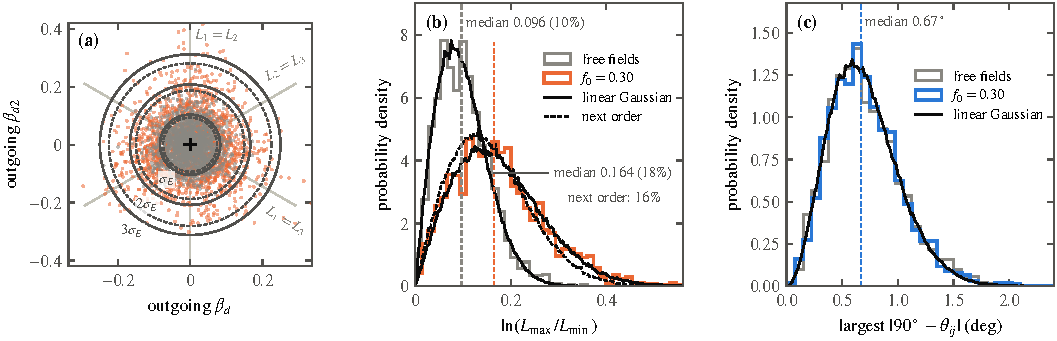
\includegraphics[width=\textwidth]{prd_fossil_shape}
\caption{Frozen shape of the torus after a Standard Model turning point. (a)~Outgoing aspect coordinates of $2048$ natural turning-point states with $\fzm=0.30$ (orange) and $2048$ for free fields (gray), evolved through the full nonlinear equations; circles: $1$, $2$ and $3\sigma_E$ of the linear prediction at leading (solid) and next order (dashed, $\sigma_E=0.0934$); gray lines: two equal sides. (b)~Logarithm of the ratio of the longest to the shortest side, $\ln(L_{\max}/L_{\min})$, and (c)~largest deviation of an edge angle from $90^\circ$, for the nonlinear draws (steps) and the linear Gaussian (lines; dashed in (b): next order).} %
\label{fig:rA-fossil}
\end{figure}

\subsection{Nonlinear evolution and corrections}
\label{rA:s-nonlinear}

Classical nonlinear shape dynamics leave the fossil of a state real at the turn intact, but they end the shape when the outgoing deformation is large.

\paragraph{Equations.}
With $K=\tfrac12\dot G$, $\sigma=G^{-1}K$ and $\mathsf Y=(L/\Lb)^3K$, the leading equations are
\begin{equation}
\dot L=HL,\qquad \dot H=2h^2-2H^2-\tfrac16\Tr\sigma^2,\qquad \dot G=2K,\qquad \dot{\mathsf Y}=2\Big(\frac{\Lb}{L}\Big)^3\mathsf YG^{-1}\mathsf Y+\Big(\frac{L}{\Lb}\Big)^3G\mathsf F,
\label{eq:rA-nl-eqs}
\end{equation}
where $\mathsf F$ is the trace-free Casimir shape force from range-adaptive Ewald sums.
The equation for $\dot H$ follows from Eq.~\eqref{eq:rA-einstein} with $\rho+\bar p=\tfrac43\rho_C$ for the traceless Casimir stress, after $\rho_C=3\MPbar^2(H^2-h^2)-\tfrac12\MPbar^2S$ is eliminated with the constraint; it holds for every shape.
The Friedmann constraint, $\det G=1$ and $\Tr G^{-1}\mathsf Y=0$ are conserved and serve as accuracy gates.

\paragraph{Standard Model forces and initial data.}
For the AAA Standard Model the force is the unimodular gradient of $Z_{\rm eff}=15Z_2(G,0)-45Z_2(G,\bm\vartheta_F)$, the 15 periodic bosonic and 45 antiperiodic Weyl degrees of freedom, which matches finite differences of $Z_{\rm eff}$ to $10^{-11}$. %
Each draw starts at the turning point with $\beta_A$ and $\Pi_A$ sampled from the Wigner function of the chosen Gaussian, $G_0=\exp(2\sum\beta_AX_A)$, the momentum $G_0^{1/2}(\sum_A\Pi_AX_A)G_0^{1/2}$ up to the normalization of Eq.~\eqref{eq:rA-delta}, and the turning-point size from the constraint at $H=0$.
A shape-independent ground energy $Q/L=\fzm C/L$ enters only through the constraint, $Z_{\rm eff}(G)\to Z_{\rm eff}(G)-\fzm Z_{\rm eff}(\rAone)$, and leaves the force unchanged; with it $\kappa_A\to\kappa_A/(1-\fzm)$ and $\delta\to\delta(1-\fzm)^{-3/4}$.
A draw survives if it reaches $ht=12$ without recollapse, with the smallest eigenvalue of $G$ above $10^{-3}$ throughout and $H>0.9\,h$ at the end. %

\paragraph{Integration and controls.}
We integrate with an eighth-order Runge--Kutta method at relative tolerance $10^{-11}$; small-amplitude runs reproduce the linear transfer to $2\times10^{-9}$, and the gates hold to $7\times10^{-11}$ for the natural states. %
Enlarging the Ewald cutoff by $40\%$, relaxing the tolerance to $10^{-9}$, or deepening the collapse criterion to $10^{-6}$ changes no fate among the draws tested. %
The evolution is a truncated Wigner approximation: it is exact at linear order and omits the Moyal terms, and the volume and inflaton are classical.
Convergence studies of these runs are collected in Sec.~\ref{rep:v-convergence}.

\paragraph{Natural states.}
We drew phase-space points from the Wigner function of the natural Standard Model state and evolved each through the full equations for $L$ and the five-dimensional $G$, with twisted Ewald forces, on the turning-point solution.
For free fields all $128$ and $2048$ draws survive, and their outgoing aspect variances exceed those of the same draws under the linear transfer by factors $1.016$ and $1.012$. %
Of 64 free-field draws with amplitudes scaled by $3$, $5$, $8$ and $12$, all, $63$, $54$ and $44$ survive, and the 2048 natural draws give $\langle\Tr B^3\rangle/\langle\Tr B^2\rangle^{3/2}=-0.07\pm0.03$ for $B=\sum\beta_{A,+}X_A$, a slight preference for two long sides and one short one. %
With $\fzm=0.30$ two sets of $2048$ draws, one reusing the normal deviates of the free-field draws and one with an independent seed, all survive, with factors $1.043$ and $1.045$ ($95\%$ intervals $1.033$--$1.054$ and $1.035$--$1.055$) for the aspect modes and $0.998$ and $1.004$ for the angle modes, and individual shapes move by $8$--$9\%$ rms ($8.6\%$ and $8.3\%$). %
The median of $\ln(L_{\max}/L_{\min})$ is then $0.164$, against $0.165$ for the linear Gaussian. %
An independent implementation gives $1.032$ ($1.023$--$1.040$); the $1.5\sigma$ difference is consistent with the convention for the initial momentum at finite amplitude. %

\paragraph{How large states fail.}
Larger states fail in one way.
The volume turns at $t\simeq0$, and then one cycle is squeezed to zero within $0.3$--$4$ Hubble times; the smallest eigenvalue of $G$ falls from $10^{-3}$ to $10^{-6}$ in at most $0.007/h$, a finite-time singularity of the shape. %
Every failure but those at the largest amplitudes is a collapse of one cycle after the volume has turned: in the independent implementation $H$ crosses zero when the smallest eigenvalue of $G$ is near $0.04$, and the eigenvalue reaches zero about $0.04/h$ later. %
The volume fails to turn only for states at least $20$ times wider than the natural one, or real at $ht_x\leq-2$, in at most $3\%$ of the draws there. %

\paragraph{Amplitude scans.}
Table~\ref{tab:rA-amp} collects the survival of the natural state scaled by $s$ at $\fzm=0.30$, from our main code with 256 draws per point, a second run with 2048 draws near the $99\%$ level, and an independent implementation with its own Ewald sums, integrator and seeds. %
Scaling the natural state by a factor $s$, the independent implementation with $2048$ draws each gives survival $1.000$, $0.987$, $0.818$, $0.365$, $0.067$ and $0.0015$ for $s=1$, $3$, $5$, $10$, $20$ and $40$, in agreement with our main runs with $256$ draws per point [Fig.~\ref{fig:rA-survival}(a)]. %
Half of the trajectories survive up to $s_{50}=8.2$ and $90\%$ up to $s_{90}=4.2$--$4.3$. %
Linear interpolation in $\ln s$ between the nodes of the 2048-draw run gives $s_{99}=2.76$ ($95\%$ interval $2.66$--$2.90$), a logistic fit $2.86$ ($2.74$--$2.96$), and the $1\%$ quantile of the critical amplification of single draws in the independent run $2.95$. %
The $99\%$ level therefore lies at $s_{99}\simeq2.8$--$2.95$, a range that spans interpolation, a logistic fit and the quantiles of the critical amplification of single draws. %
The 2048-draw value of $S(3)$, $0.9834\pm0.0028$, and the independent $0.987$ differ by about $2\sigma$, which accounts for the spread. %
In terms of the outgoing linear amplitude, $99\%$ of the trajectories survive below $\sigma_{\rm lin}\simeq0.29$--$0.31$ per aspect mode, and half below $0.85$--$0.89$. %
At next order the same procedure gives $s_{99}=3.16$ (logistic $3.29$), $s_{90}=4.19$ and $s_{50}=9.07$. %
Free fields tolerate more: every draw survives up to three times the natural amplitude, while with $\fzm=0.30$ that amplitude keeps $97$--$99\%$ of the trajectories. %

\begin{table}[tbp]
\centering
\caption{Survival of the natural turning-point state scaled by $s$, at $\fzm=0.30$: runs of our main code with 256 and 2048 draws per point, an independent implementation with 2048 draws, and the rms outgoing aspect amplitude $\sigma_{\rm lin}$ of the linear images of the sampled draws.}
\label{tab:rA-amp}
\begin{tabular}{lcccc}
\toprule
$s$ & 256 draws & 2048 draws & independent & $\sigma_{\rm lin}$\\
\midrule
1 & 1.000 & --- & 1.000 & 0.109\\ %
2.5 & --- & 0.9976 & --- & 0.262\\ %
3 & 0.973 & 0.9834 & 0.987 & 0.314\\ %
3.5 & --- & 0.9536 & --- & 0.366\\ %
5 & 0.824 & --- & 0.818 & 0.543\\ %
10 & 0.367 & --- & 0.365 & 1.085\\ %
20 & 0.062 & --- & 0.067 & 2.171\\ %
40 & 0.000 & --- & 0.0015 & 4.342\\ %
\bottomrule
\end{tabular}
\end{table}

\paragraph{One survival curve.}
Survival is mainly a function of $\sigma_{\rm lin}$.
For $\sigma_{\rm lin}\lesssim1.5$ the amplitude scans at three stiffnesses, the real states of Sec.~\ref{rA:s-conditional}, the phase and adiabatic families and the outgoing never-real states lie on one curve to within $\pm5$ percentage points. %
The comparison of Tables~\ref{tab:rA-S2} and~\ref{tab:rA-amp} shows the same: a real state at $h|t_x|=0.25$ has $\sigma_{\rm lin}=0.297$ and survives with $0.987$, as does the natural state scaled by $s=3$, with $\sigma_{\rm lin}=0.314$.

\begin{figure}[tbp]
\centering
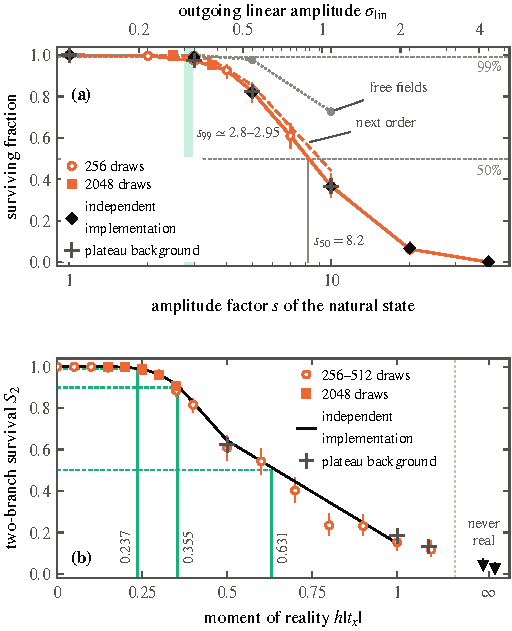
\includegraphics[width=0.8\textwidth]{prd_nonlinear_survival}
\caption{Shape survival through a Standard Model turning point with $\fzm=0.30$. (a)~Surviving fraction when the natural turning-point state is scaled by $s$: runs with $256$ and $2048$ draws per point, an independent implementation (diamonds), the same draws on the $A_s$-calibrated plateau background (crosses), next order (dashed), and free fields (dotted); upper axis: outgoing linear amplitude $\sigma_{\rm lin}$; band: $s_{99}\simeq2.8$--$2.95$. (b)~Two-branch survival $S_2$ of the optimal real Gaussian versus the moment of reality $h|t_x|$, with an independent implementation (line), plateau-background states (crosses), never-real pairs ($\infty$), and the thresholds $0.237$, $0.355$, and $0.631$ for $99\%$, $90\%$, and $50\%$. Wilson $95\%$ intervals.} %
\label{fig:rA-survival}
\end{figure}

\paragraph{Moyal correction.}
Quantum corrections are small.
Expanding $Z_{\rm eff}/Z_{\rm eff}(\rAone)$ to third order at the cube, with tensor $c_{ABC}$, the second moments of the quantum and the truncated Wigner evolution differ first at order $c^2$, through the third-derivative term of the Moyal bracket:
\begin{equation}
\Delta\rAVar\,q_A=-\frac{\delta^2}{2}\iint dt\,dt'\,W_A(t)W_A(t')\sum_{BC}c_{ABC}^2\,r_B(t,t')\,r_C(t,t'),
\end{equation}
with $r_B(t,t')=f_B(t)g_B(t')-g_B(t)f_B(t')$ built from the fundamental solutions $f,g$ of each mode, $W_A(t)=V(t)\,r_A(T,t)$ and $V=-3/(cL)$ in the units of Sec.~\ref{rA:s-quantization}.
The correction depends on the window over which the state evolves quantum mechanically, not on the initial state, and quartic terms give no quantum-classical difference at this order.
For the AAA Standard Model at $\fzm=0.30$ the three independent cubic constants are $c_{E^3}=12.50$, $c_{ET_2^2}=7.91$ and $c_{T_2^3}=-5.57$, five times those of the Maxwell toy. %
For the Standard Model with a state real at the turn it changes the aspect variance by $-0.020\%$ and the angle variance by $-0.11\%$. %
This is $28$ times less than for the Maxwell toy prepared twelve Hubble times before the turn; on that window the Standard Model value is $-1.0\%$. %
For real states set before the turn it is $-0.07\%$ to $-0.51\%$. %
An independent implementation reproduces the earlier Maxwell-toy coefficient to $1.2\times10^{-7}$, and an exact split-operator evolution of a single mode agrees with the formula to $0.35\%$, $1.4\%$ and $5.8\%$ at half, one and two times the Standard Model coupling, a deviation that grows as $c^2$. %
At next order the aspect and angle corrections become $-1.79\times10^{-4}$ and $-9.2\times10^{-4}$. %
These bounds concern second moments; the survival fractions, set by trajectories near collapse, are not constrained by them.

\paragraph{Plateau background.}
To test the leading solution we replaced it by the time-symmetric plateau history with a homogeneous rolling inflaton, $\hat V(\phi)=3[(1-e^{-a\phi})/(1-e^{-a\phi_b})]^2$ with $a=\sqrt{2/3}$ and $\phi_b=5.5794$, in units of $\MPbar^2\rAHeff^2$. %
The turning-point data at $t=0$ are identical, and for $\phi_b\to\infty$ the code reproduces the leading-solution runs to $1.4\times10^{-14}$. %
Replacing the leading turning-point solution by this history changes the linear gains by $+3$--$4\times10^{-4}$ and, in $2560$ trajectories paired with the leading-solution runs, at $s=1$, $3$, $5$ and $10$ and for real states at $ht_x=-0.5$, $-1$ and the onset of freezing, the fate of none. %
The outgoing shapes of common survivors differ by a median of $1.5$--$3.4\times10^{-4}$ in relative terms. %
The independent implementation, run on a second reference plateau with $\phi_b=5.587$, finds survival higher by $0.4$--$0.8$ percentage points, all from draws that survive on the plateau and fail on the leading solution. %
For the Maxwell toy the backreaction of the shape moments on the volume and inflaton shifts $N_{\rm post}$ by $-5\times10^{-4}$ and the aspect variance by $+0.05\%$. %

\paragraph{Shear criterion.}
At the turning point $H=0$, and the constraint fixes $u\equiv(L/\Lb)^2$.
With $\zeta=Z_{\rm eff}(G_0)/Z_{\rm eff}(\rAone)$ and $s_0=\Tr[(G_0^{-1}\mathsf Y_0)^2]$ in the units of Eq.~\eqref{eq:rA-nl-eqs}, the shear at the turn is $S=s_0h^2/u^3$ and the constraint, multiplied by $u^2/3\MPbar^2h^2$, reads
\begin{equation}
u^2+\frac{s_0}{6u}=\zeta .
\end{equation}
The left side has its minimum $3(s_0/12)^{2/3}$ at $u^3=s_0/12$, so a large-volume root exists if and only if $s_0\leq12(\zeta/3)^{3/2}$.
Along a single direction this predicts the critical momentum $p_c=1.43276$, and the integration turns at $0.99\,p_c$ and fails at $1.01\,p_c$. %
Near the cube, $\zeta\simeq1$, the criterion is $\rho\equiv s_0/12<3^{-3/2}=0.19245$: a trajectory has turning-point data only if its shape momenta obey $\sum_AP_A^2<12\cdot3^{-3/2}\,\MPbar^4\Lb^6\rAHeff^2$. %
States set in an adiabatic vacuum ($\omega=c_\omega|H|$) at the onset of the plateau contraction violate it on average after $N_{\rm pre}=1.32$ ($c_\omega=1$) and $1.01$ ($c_\omega=3$) e-folds of contraction, whereas optimal-width real states keep the mean ratio below $0.112$. %
For fixed shape momenta, which are conserved across the thin turning layer, the volume obeys the Wheeler--DeWitt equation
\begin{equation}
\psi''(x)+12X^2\Big[3e^{6x}-3\zeta e^{2x}+\frac{s_0}2\Big]\psi=0,\qquad x=\ln(L/\Lb),
\end{equation}
which is Eq.~\eqref{eq:rA-WDWeq} with $6p_\beta^2\to6s_0X^2$.
A uniform parabolic-cylinder approximation gives the collapse probability $1/\{1+\exp[24.81X(\rho_c-\rho)]\}$, which numerical scattering confirms for $X=30$--$2282.49$ with errors falling as $1/X$. %
At $X=2282.49$ the criterion moves by $3.5\times10^{-8}$ in relative terms, and its 10--90\% width is $\Delta\rho=7.8\times10^{-5}$, or $4\times10^{-4}$ relative. %
A quantum treatment of the volume therefore turns the classical step into a smooth one of relative width $4\times10^{-4}$ without moving it. %

\subsection{Why a Euclidean continuation does not fix the state}
\label{rA:s-euclid}

A no-boundary prescription is the natural candidate for selecting the turning-point state.
Continuing $t=-i\tau$, $\tanh2ht\to-i\tan2h\tau$, ${\rm sech}^22ht\to\sec^22h\tau$ and $d/dt\to i\,d/d\tau$, Eq.~\eqref{eq:rA-shapeode} becomes
\begin{equation}
\beta''-3h\tan(2h\tau)\beta'+\kappa h^2\sec^2(2h\tau)\beta=0 .
\end{equation}
This reaches the singular end $L_E=\Lb\sqrt{\cos2h\tau}\to0$ of the Euclidean solution, at $h\tau_0=\pi/4$, which Ref.~\cite{Guth:2025dal} rejects as an instanton.
Near that end, with $s=\tau_0-\tau\to0$, $\tan2h\tau\simeq1/2hs$ and $\sec^22h\tau\simeq1/4h^2s^2$, and the continued equation becomes
\begin{equation}
\beta_{ss}+\frac{3}{2s}\beta_s+\frac{\kappa}{4s^2}\beta=0,
\end{equation}
with solutions $s^p$ and exponents
\begin{equation}
p=-\tfrac14\pm\tfrac14\sqrt{1-4\kappa}.
\end{equation}
The quadratic action $\tfrac12\int ds\,(s^{3/2}\beta_s^2-\tfrac\kappa4s^{-1/2}\beta^2)$, whose Euler--Lagrange equation is the one above, reduces on shell to the boundary term $\tfrac12s^{3/2}\beta\beta_s\propto s^{2p+1/2}$.
For $\kappa<1/4$ only the larger exponent keeps it finite and selects the state.
For $\kappa>1/4$ both have ${\rm Re}\,p=-1/4$ and oscillate log-periodically with the same amplitude, with period $\Delta\ln s=8\pi/\sqrt{4\kappa-1}$.
The kinetic and potential parts each diverge logarithmically, but their sum stays bounded and oscillates without a limit at the singular end, so regularity selects neither solution.
A direct integration toward $\tau_0$ reproduces the predicted number of sign changes for $\kappa=6.0$, $13.5$ and $8/5$ and finds none for $\kappa\leq1/4$. %
Since some $\kappa_A\geq8/5$, every Casimir turning point has such a mode, and the Euclidean continuation of the isotropic turning point selects no shape state.
Real tunneling geometries, compact Euclidean geometries joined to Lorentzian ones across a surface of vanishing extrinsic curvature, carry the no-boundary predictions for the large-scale topology~\cite{Gibbons:1990ns}; the turning point has $K_{ij}=0$, but its singular Euclidean continuation is not of this kind.

The no-boundary saddles of a three-torus found in Ref.~\cite{Godet:2026gqw} are complex, cap one cycle smoothly and have no turning point.
Joining such a cap to the Casimir turning point needs the one-loop stress on a cigar times a two-torus, where the homogeneous Casimir formula fails.
That failure marks the precision of the homogeneous model rather than an obstruction: the stress in the flat core is finite, and on a curved cigar the negative aspect kernel keeps its sign (Sec.~\ref{rep:v-conditional}).
Whether a self-consistent capped saddle exists, and where it would center the shape, remains open.
A classical offset of the mean shape grows by $m_{11}=10.6$ through the turn, so it must stay below about $0.01$, or $1.4$ quantum widths of the natural state ($\beta_{\rm rms}=0.0071$), for the quantum fossil to dominate. %
